\let\negmedspace\undefined
\let\negthickspace\undefined
\documentclass[journal,12pt,twocolumn]{IEEEtran}
\usepackage{cite}
\usepackage{amsmath,amssymb,amsfonts,amsthm}
\usepackage{algorithmic}
\usepackage{graphicx}
\usepackage{textcomp}
\usepackage{xcolor}
\usepackage{txfonts}
\usepackage{listings}
\usepackage{enumitem}
\usepackage{mathtools}
\usepackage{gensymb}
\usepackage{comment}
\usepackage[breaklinks=true]{hyperref}
\usepackage{tkz-euclide}
\usepackage{listings}
\usepackage{gvv}
\def\inputGnumericTable{}
\usepackage[latin1]{inputenc}
\usepackage{color}
\usepackage{array}
\usepackage{longtable}
\usepackage{calc}
\usepackage{multirow}
\usepackage{hhline}
\usepackage{ifthen}
\usepackage{lscape}
\usepackage{circuitikz}

\newtheorem{theorem}{Theorem}[section]
\newtheorem{problem}{Problem}
\newtheorem{proposition}{Proposition}[section]
\newtheorem{lemma}{Lemma}[section]
\newtheorem{corollary}[theorem]{Corollary}
\newtheorem{example}{Example}[section]
\newtheorem{definition}[problem]{Definition}
\newcommand{\BEQA}{\begin{eqnarray}}
\newcommand{\EEQA}{\end{eqnarray}}
\newcommand{\define}{\stackrel{\triangle}{=}}
\theoremstyle{remark}
\newtheorem{rem}{Remark}
\begin{document}

\bibliographystyle{IEEEtran}
\vspace{3cm}

\title{Gate 2021- Instrumentation Engineering}
\author{EE23BTECH11058 - Sindam Ananya$^{*}$% <-this % stops a space
}
\maketitle
\newpage
\bigskip

\renewcommand{\thefigure}{\theenumi}
\renewcommand{\thetable}{\theenumi}

\vspace{3cm}
\textbf{Question 43:} 
Given $y(t) = e^{-3t}u(t) * u(t+3)$, where * denotes convolution operation. The value of $y(t)$ as $t \rightarrow \infty$ is
\hfill{(GATE IN 2021)}\\
\solution
\begin{align}
y(t) &=  e^{-3t}u(t) * u(t+3)\\
x(t) &\xleftrightarrow{\mathcal{F}} X(j\omega)\\
x(t-t_o) &\xleftrightarrow{\mathcal{F}} e^{-j\omega t_o}X(j\omega)\\
x_1(t) * x_2(t) &\xleftrightarrow{\mathcal{F}} X_1(j\omega)X_2(j\omega)\\
e^{-at} &\xleftrightarrow{\mathcal{F}} \frac{1}{j\omega + a}\\
u(t) &\xleftrightarrow{\mathcal{F}} \frac{1}{j\omega}\\ 
Y(j\omega) &= \brak{\frac{1}{j\omega + 3}}\brak{\frac{e^{3j\omega}}{j\omega}}
\end{align}
By solving through partial fractions,
\begin{align}
Y(j\omega) = \frac{e^{3j\omega}}{3j\omega} - \frac{e^{3j\omega}}{3\brak{j\omega+3}} 
\end{align}
By applying inverse fourier transform,
\begin{align}
y(t) = \frac{u(t+3)}{3} - \frac{e^{-3t}u(t+3)}{3}
\end{align}
As $t \rightarrow \infty $, $e^{-at} \rightarrow 0$ \quad \brak{a > 0}
\begin{align}
y(t) &= \frac{1}{3} \\
     &= 0.33
\end{align}
\begin{figure}[h!]
    \centering
    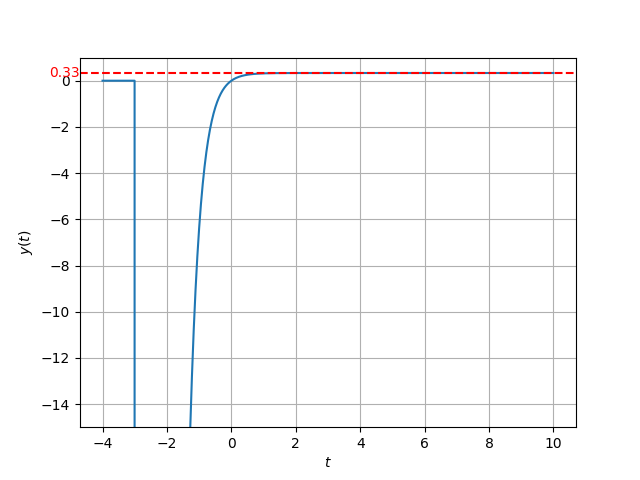
\includegraphics[width=0.8\columnwidth]{figs/plot.png}
    \caption{plot of $y(t)$}
    \label{fig:gate202138fig}
\end{figure}
\end{document}
